\documentclass[UTF8, twoside]{EPURapport}
\usepackage{algpseudocode}
\usepackage{algorithm}
\usepackage{pdfpages}
\usepackage[nottoc, notlof, notlot]{tocbibind}
\usepackage{amsmath,amsfonts,amsthm}
\usepackage{graphicx}
\usepackage{rotating}
\usepackage{color}
\usepackage{colortbl}
%\usepackage{listings}

%\renewcommand{\lstlistlistingname}{Liste des codes}
%\renewcommand{\lstlistingname}{Code}

%\addextratables{%
%	\lstlistoflistings
%}

%\swapAuthorsAndSupervisors



\thedocument{Operational research project draft}{Ant colony optimization algorithm for a combined routing and scheduling problem}{Ant colony optimization algorithm for a combined routing and scheduling problem}

\grade{Computer Aided Decision Support\\ International Research Master 2\\ 2013 - 2014}

\authors{%
	\category{Student}{%
		\name{Thomas NOGUER} \mail{thomas.noguer@etu.univ-tours.fr}
	}
	\details{M2RI CADS 2013 - 2014}
}

\supervisors{%
	\category{Supervisors}{%
		\name{Jean-Charles BILLAUT} \mail{jean-charles.billaut@univ-tours.fr}
		\name{Nicolas MONMARCHÉ} \mail{nicolas.monmarche@univ-tours.fr}
	}
	\details{Université François-Rabelais, Tours}
}

\abstracts{abstract}
{keywords}

\begin{document}

\chapter{Formalization of the problem}

	The problem can be defined from three different sub-problems :
	
\begin{itemize}
\item[$\bullet$] The two machines permutation flowshop. We have two machines $M_1$ and $M_2$ organized as a flowshop. A set of $n$ jobs have to be scheduled into a sequence. Each job $j$ has a value $a_j$ and $b_j$ that correspond to the time required to complete the job $j$ on $M_1$ and $M_2$ respectively.
\item[$\bullet$] The grouping of jobs to be delivered. When the jobs are completed for the two machines permutation flowshop we must form groups of jobs, where a group must contain at least one job. These groups are then used for the third sub-problem.
\item[$\bullet$] A travelling salesman problem. We consider one truck taking the group of jobs previously formed where each job has a destination $k_j$. The idea is to find the sequence of destinations in order to deliver every job from the group while minimizing the travelling distance. We have a matrix $K$ ($m \times m$) where $m$ is the number of destinations and $K_i^j$ is the distance between the destination $i$ and $j$.
\end{itemize}

	The objective function is to minimize the sum of tardiness of the jobs $\overset{j \leq n}{\underset{j=1}{\sum}} T_j$. The tardiness $T_j$ of a job is defined as follows: $T_j = max(L_j, 0)$ where the lateness $L_j$  of a job $j$ is the difference between the completion time of the job $c_j$ and its due date $d_j$: $L_j = c_j - d_j$. The completion time of a job is not equal to the completion time of the job for the flowshop problem but for the travelling salesman problem. \textbf{$c_j$ is equal to the date at which the truck is coming back to the factory after its deliveries.}
\textbf{We consider that the truck has no capacity limit, it can carry has many jobs has possible.}
\\

	The input data of our problem are the following :
\begin{itemize}
\item[$\bullet$] The number $n$ of jobs,
\item[$\bullet$] The values $a_j$, $b_j$ and $d_j$ of job $j$ ($\forall j \in [1,n]$),
\item[$\bullet$] The number of $m$ destinations,
\item[$\bullet$] The destination $k_j$ of job $j$ ($\forall j \in [1,n]$),
\item[$\bullet$] The matrix $K$ ($m \times m$) of distances between each destination.\\
\end{itemize}

	During the resolution of the problem we must find the sequence of jobs on the flowshop, the groups of jobs to be delivered and the sequence of delivery for each group.

	We proposed a first way of encoding a solution : a table of size $n$ containing the sequence of job for the flowshop sub-problem, a table of size $2n$ containing the groups and sequences for the travelling salesman sub-problem. The first cell of the second table contains the number of jobs for the first group, the following cells contain the number of jobs in the delivery sequence and so on. The figure \ref{problem} shows a solution for a simple instance of the problem with its encoding. 
	
	The sequence here is $\{1,2,3\}$ the first group $G_1$ of jobs is $G_1 = \{1,2\}$ and 1 is delivered first, the second group $G_2$ only contains one job $G_2 = \{3\}$.
	
	
\begin{figure}
	\centering 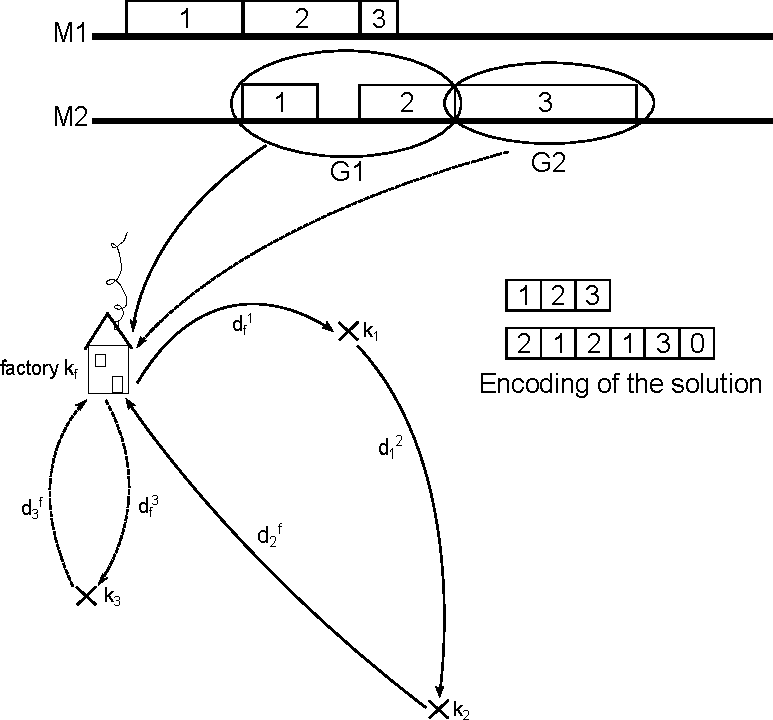
\includegraphics{images/problem.pdf}
	\caption {A solution of the problem for a simple instance}	
	\label {problem}
\end{figure}

\chapter{Ant colony optimization}

\section{General definitions}

 	\hspace{4ex}In this first part we will consider a travelling salesman problem in order to explain the mechanism of the ant colony metaheuristic. The graph representation of cities is an intuitive approach for such a method.
	
	
	The classic algorithm of an ant colony heuristic is the following :

\begin{algorithm}
  \caption{Ant colony}
  \begin{algorithmic}[1]
      \For{$k \gets 1 \textrm{ to } iterationsNumber$}
      	\For {\textbf{each} $ant$}
        	\State Construct solution
			\State Local pheromone update
        \EndFor
        \State Local search
        \State Global pheromone update
      \EndFor
      \State \textbf{return} Best found solution
  \end{algorithmic}
\end{algorithm}

	In order to construct the solution we need a probability formula based on the following :
	\\

\[
P^m_{}ij= \left\{ 
\begin{array}{l r}
\frac{[\tau_{ij}]^\alpha \cdot [\eta_{ij}]^\beta}{\underset{l\notin tabu_m}{\sum}[\tau_{il}]^\alpha \cdot [\eta_{il}]^\beta} & \text{if } j\notin tabu_m\\
0 & \text{if } j\in tabu_m
\end{array}
\right.
\]

	Where $P^m_{ij}$ is the probability of an ant $m$ in city $i$ to go to the city $j$, $\tau{ij}$ the intensity of the pheromone trail from $i$ to $j$, $\eta_{ij}$  the visibility of city $j$ from city $i$ (this is typically $1/d_{ij}$ where $d_{ij}$ is the distance between $i$ and $j$). $\alpha$ and $\beta$ are parameters used to make the pheromone trail or the visibility more important from one another. And finally, the tabu list is used to prevent ants from going to forbidden cities like the city they come from.
\\

	The local pheromone update is used to emulate the evaporation phenomenon of pheromone. This evaporation is calculated from a formula based on the following :
	\\
	
\[
\tau_{ij} = (1-\rho) \cdot \tau_{ij}+\rho \cdot \tau_{min}
\]

	Where $\rho$ is the evaporation rate and $\tau_{min}$ the minimum value of the pheromone trail, which is also usually used as initial value. \textbf{It is important to consider that the evaporation function is only used for the paths the ants travelled through.}
\\

	The global pheromone update is used to emulate the deposit of pheromone from the ants. This deposit is calculated from a formula based on the following :
	\\
	
\[
\tau_{ij} = (1-\rho) \cdot \tau_{ij}+\rho \cdot \Delta\tau_{ij}
\]

	Where $\Delta\tau_{ij}$ can be defined as follows :
	\\
	
\[
\Delta\tau_{ij} = \left\{ 
\begin{array}{l l}
15 & \text{if } (i,j) \text{ is an edge in the best and second best,}\\
10 & \text{if } (i,j) \text{ is an edge only in the best,}\\
5 & \text{if } (i,j) \text{ is an edge only in the second best}\\
\end{array}
\right.
\]

\section{Application to the combined routing and scheduling problem}

	\hspace{4ex}One main issue to overcome here is the fact that there is no simple graph representation of the complete problem. For the travelling salesman problem, it is easy to see how the pheromone trails and the visibility comes from. For our problem it is quite different. We can try to imagine a graph that an ant could visit and form a complete solution from it. For instance, a node could represent the fact that a job $j$ is placed first in the flowshop, alone in a delivery group and delivered first. But we then have to consider every possibility knowing that the grouping and delivering problems are dependant on the flowshop. If we change the sequence of jobs in the flowshop we obtain a different grouping problem and then a different travelling salesman problem.
	
	Even though we happen to be able to model such graph, its size would be unreasonably huge. It is not rational to chose such solution. \textbf{We must abandon the idea to apply the ant colony optimization all at once for our problem, we need to think of a different approach.}
	\\
	
	Instead of trying to use the ant colony metaheuristic for the complete problem, we can consider using it for parts of it. \textbf{We can chose to use the ant colony on one or several sub-problem and use different method to construct the rest of the solution and then update the pheromone trails based on the results of the whole solution.} 
	
	Although is not clever to consider using the ant colony for the travelling salesman sub-problem since the problem is different each time you change the groups to be delivered or the sequence of jobs from the flowshop. The pheromone trails would be lost each time you change the solution in any sub-problem above.
	
	We can still consider the other two sub-problems as potential candidate for the ant colony. Indeed, the flowshop problem and the grouping problem can both be considered central in our global problem. \textbf{We then have three possibilities, use the ant colony on the flowshop, on the grouping problem or both and use simple heuristics coupled with a surrogate mechanism to obtain the value of the objective function for our solution in order to guide the ants towards the best solution.} The surrogate mechanism could be very useful in order to save time computation, it would be used in the majority of cases and replaced with heuristics in the others in order to verify if the current solution is still a good one.
\\	

\subsection{Definition of the Ant colony for the mixed optimisation problem}
	
	Here we decided to use the ant colony metaheuristic on the grouping problem. It is easy to find heuristics to construct the rest of the solution when we have the groups of jobs. We have to specify how to implement the ant colony algorithm to our sub-problem. This typical visualisation we use for an ant building a solution of the travelling salesman problem is a complete graph. The nodes of the graph are cities, when the ant goes from city $a$ to city $b$ is means we have the sequence $ab$ in our solution. The ant has to visit all nodes with a specific path. It chooses a path from the probability formula defined before.
	
	We use a different construction of solution for our algorithm. We take the jobs as the nodes of the graph and two edges (a green and a red) connect each node together. The graph has then $n$ nodes and $n(n+1)$ edges. During the construction of a solution, and ant can come from a node $a$ to a node $b$ from two different edges: If it takes the green edge it means node $a$ and $b$ belong to the same group, if it takes the red edge it means the two nodes don't belong to the same group. The figure \ref{ant_colony_graph} shows how to construct the groups from the path travelled by an ant on our graph.
\\

\begin{figure} [h]
	\centering 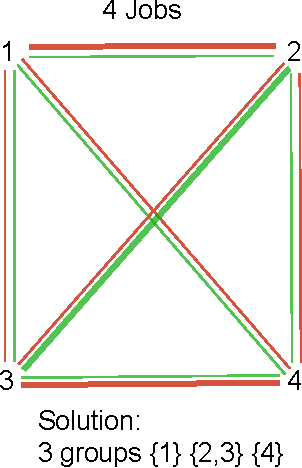
\includegraphics{images/ant_colony_graph.pdf}
	\caption {The construction of a solution by an ant.}	
	\label {ant_colony_graph}
\end{figure}

	We know how the ants construct the solution and how the graph is made. What we need is to define the visibility criterion for each arc of our graph. Let's define the visibility for the green edges, what is the formula that will make the ants form groups of jobs? We are handling a complex problem, we need to take into account the two other sub-problems: the flowshop, and the travelling salesman.
\\
	
	For the travelling salesman what we wish to do is group the jobs is their distance is small: $\frac{1}{\delta_{ij}}$ where $\delta_{ij}$ is the distance between the destination of job $i$ and the destination of job $j$. 
	
	For the deliveries we know that we have to start from the factory and to end at the factory, the distance between the destinations of the jobs and the factory matters, when the jobs are far from the factory we tend to form groups: $\frac{\delta_{0i} \cdot \delta_{0j}}{\delta_{max}}$ where $\delta_{0i}$ is the distance between the factory and the destination of job $i$ and $\delta_{max}$ is the maximum distance between the factory and any other destination. We divide by the maximum value in order to keep a value between 0 and 1.
	
	We can then combine those two criteria and add a tuning parameter $\omega$ to make one criterion or the other more important: 
\\

\[
\left(\frac{1}{\delta_{ij}}\right)^\omega \cdot \frac{\sqrt{\delta_{0i} \cdot \delta_{0j}}}{\delta_{max}}
\]
\\

\textbf{With this criterion, we will form groups of jobs the further their destinations are from the factory and the closer their destinations are from one another.}
\\

	For the flowshop sub-problem we want to consider the due dates of the jobs. \textbf{When the due dates of two jobs are close to each other we will tend to put them into the same group}: 
\\

\[
\frac{1}{\vert d_i - d_j \vert}
\]
\\

	We can combine the criterion from both sub-problem, add tuning parameters and get the formula of the visibility $\eta_{ij}$:
\\

\[
\eta_{ij} = 
\left( \frac{1}{\vert d_i - d_j \vert} \right)^\psi \cdot \left[\left(\frac{1}{\delta_{ij}}\right)^\omega \cdot \frac{\sqrt{\delta_{0i} \cdot \delta_{0j}}}{\delta_{max}} \right]^\chi \text{, where } \vert d_i - d_j \vert \neq 0 \text{ and } \delta_{ij} \neq 0
\]
\\

	We said before that this visibility was to be considered for the green edges of our graph. The visibility $\eta_{ij}^{-1}$ for the red edges take the inverse criteria of the visibility of the green edges:
\\

\[
\eta_{ij}^{-1} = \frac{1}{\eta_{ij}} =
\left( \vert d_i - d_j \vert \right)^\psi \cdot \left[\left(\delta_{ij}\right)^\omega \cdot \frac{\delta_{max}}{\sqrt{\delta_{0i} \cdot \delta_{0j}}} \right]^\chi \text{, where } \delta_{0i} \cdot \delta_{0j} \neq 0 
\]
\\
	
\textit{Explain here the point of the roulette and how it is defined}

\subsection{Algorithms}

	Let us call our search graph $G$, the node set of this graph $\mathscr{N}$, the green edge set $\mathscr{G}$ and the red edge set $\mathscr{R}$. 

\begin{algorithm}
  \caption{Ant colony for the mixed optimisation problem}
  \begin{algorithmic}[1]
  	  \State Initialize pheromone matrix with $\tau_0$
  	  \State Calculate the matrix of visibility
  	  \State List $path$
      \For{$k \gets 1 \textrm{ to } iterationsNumber$}
      	\For {\textbf{each} $ant$}
      		\State \textit{/* Construction of the solution for the grouping problem*/}
			\State Select random node $u$ from $\mathscr{N}$
    		\State $i \gets 1$
    		\Repeat
    			\State Pick a random number $p \in \{0,1\}$
    			\If {$p < P_0$}
    				\State From all incident edges of $u$ get $v$ the edge with the maximum value of $P_{uv}$
    				
				\Else
					\State \textit{Select edge v from roulette}
    			\EndIf
    			\If {$v \in \mathscr{G}$}
   					\State $path.push(v)$
   				\EndIf
   				\State $i \gets i+1$
    		\Until $i = n$
    		\State Each community of nodes linked with edged from $path$ form a group
    		\State Each remaining nodes form an individual group containing only this node
    		\State \textit{/* Construction of the rest of the solution */}
    		\State Use heuristics to construct the rest of the solution
    		\State Computation of $\underset{i}{\sum} T_i$
    		\If{the new solution is better than the best known solution}
    			\State Save the new solution as the new best known solution
    		\EndIf
			\State Local pheromone update
        \EndFor
        \State Local search
        \State Global pheromone update
      \EndFor
      \State \textbf{return} Best found solution
  \end{algorithmic}
\end{algorithm}

\clearpage

	When we have forms the batches of jobs we have to deduce the rest of the solution. In order to do so we will use heuristics. For the flowshop problem we select the order of batch in increasing order of the minimum of the due date of each batch. Each batch is then scheduled following Johnson's algorithm.
	
	For the travelling salesman problem we find the sequence of destination of each batch by using the closest neighbour criterion with each subset of jobs formed by our groups.



\end{document}
